\documentclass[preprint,12pt]{elsarticle}
\usepackage{booktabs}
\usepackage{amsmath,amssymb}
\usepackage{graphicx}
\usepackage{hyperref}
\usepackage{xcolor}

\journal{Neurocomputing}

\begin{document}
\begin{frontmatter}
\title{Physics-Guided Satellite Data Assimilation with Ablation-Oriented Evaluation}
\author{Liu Ruixin}
\address{School of Automation, Southeast University, Nanjing, China}
\begin{abstract}
This draft reports an ablation-oriented neural assimilation pipeline. We evaluate model accuracy, computational overhead, and statistical significance.
\end{abstract}
\begin{keyword}
Satellite data assimilation \sep Neural network \sep Ablation study \sep Statistical significance
\end{keyword}
\end{frontmatter}

\section{Results}
\begin{table}[t]
\centering
\caption{Overall comparison on test set.}
\resizebox{\textwidth}{!}{%
\begin{tabular}{llccccccc}
\toprule
Method & Type & RMSE & MAE & Bias & Corr & Improve(\%) & Params(M) & GFLOPs\\
\midrule
Background (ERA5) & bkg & 1.8230 & 1.2177 & +0.0020 & 0.99624 & +0.00 & -- & --\\
OI/1DVar (B2) & oi & 1.8836 & 1.2798 & -0.0014 & -- & -3.32 & -- & --\\
Ours-ours\_with\_full & ours & 1.1081 & 0.7726 & +0.0645 & 0.99878 & +39.22 & 27.69 & 4.79\\
Ablation-v1\_noaux\_mse & ablation & 1.1867 & 0.8206 & +0.0424 & 0.99855 & +34.91 & 27.69 & 4.79\\
Ablation-v2\_noaux\_no\_deep\_supervision\_64 & ablation & 1.2247 & 0.8470 & +0.0847 & 0.99853 & +32.82 & 27.69 & 4.79\\
Ablation-v3\_fusion\_add\_no\_deepsupervision\_64 & ablation & 1.2809 & 0.8795 & +0.0658 & 0.99818 & +29.74 & 27.69 & 4.79\\
Ablation-v4\_noaux\_spectral\_stem\_64 & ablation & 1.6160 & 1.1074 & +0.0894 & 0.99672 & +11.35 & 27.70 & 4.89\\
Ablation-v5\_noaux\_no\_mask\_aware\_64 & ablation & 1.1883 & 0.8177 & +0.0588 & 0.99863 & +34.82 & 27.69 & 4.81\\
Ablation-v6\_noaux\_no\_mask\_aware\_64 & ablation & 1.2851 & 0.8822 & +0.0933 & 0.99830 & +29.51 & 27.69 & 4.81\\
Baseline-compare\_b10\_with\_mamba & compare & 1.1246 & 0.7806 & +0.0332 & 0.99871 & +38.31 & 27.69 & 4.79\\
Baseline-compare\_b3\_vanilla\_unet\_64 & compare & 1.4469 & 1.0060 & +0.1450 & 0.99696 & +20.63 & 13.28 & 6.37\\
Baseline-compare\_b4\_fuxi\_da\_64 & compare & 1.3396 & 0.9471 & +0.1038 & 0.99694 & +26.52 & 5.93 & 11.54\\
Baseline-compare\_b4\_fuxi\_da\_64\_tttf & compare & 1.2739 & 0.8989 & +0.0981 & 0.99752 & +30.12 & 5.95 & 11.71\\
Baseline-compare\_b5\_attn\_unet\_64 & compare & 1.4911 & 1.0364 & +0.1622 & 0.99681 & +18.21 & 17.49 & 4.61\\
Baseline-compare\_b6\_pixel\_mlp\_64 & compare & 1.6959 & 1.1654 & +0.1388 & 0.99628 & +6.97 & 0.09 & 0.73\\
Baseline-compare\_b7\_res\_unet\_64 & compare & 1.5470 & 1.0795 & +0.2046 & 0.99643 & +15.14 & 26.52 & 6.48\\
Baseline-compare\_b9\_fengwu\_64 & compare & 1.2746 & 0.8837 & +0.1429 & 0.99756 & +30.08 & 5.81 & 10.55\\
\bottomrule
\end{tabular}%
}
\end{table}


\subsection{Layer-wise Performance}
\begin{table}[htbp]
\centering
\caption{RMSE by atmospheric layer group (K). Strat: 1--100\,hPa; Trop: 100--500\,hPa; Low: 500--1000\,hPa.}
\begin{tabular}{llcccc}
\toprule
Method & Type & Stratosphere & Troposphere & Lower Trop. & Global \\
\midrule
Background (ERA5) & bkg & 2.1357 & 1.5314 & 2.3039 & 2.0506 \\
OI/1DVar (B2) & oi & 2.2158 & 1.5603 & 2.3333 & 2.0954 \\
Ours-ours\_with\_full & ours & 1.0374 & 0.7903 & 1.4371 & 1.1588 \\
Ablation-v1\_noaux\_mse & ablation & 1.1439 & 0.8624 & 1.5675 & 1.2673 \\
Ablation-v2\_noaux\_no\_deep\_supervision\_64 & ablation & 1.1686 & 0.8705 & 1.5787 & 1.2813 \\
Ablation-v3\_fusion\_add\_no\_deepsupervision\_64 & ablation & 1.3594 & 0.9441 & 1.7445 & 1.4311 \\
Ablation-v4\_noaux\_spectral\_stem\_64 & ablation & 1.9598 & 1.3531 & 2.0674 & 1.8490 \\
Ablation-v5\_noaux\_no\_mask\_aware\_64 & ablation & 1.0664 & 0.8322 & 1.5618 & 1.2381 \\
Ablation-v6\_noaux\_no\_mask\_aware\_64 & ablation & 1.2885 & 0.9388 & 1.6722 & 1.3745 \\
Baseline-compare\_b10\_with\_mamba & compare & 1.0664 & 0.8043 & 1.4722 & 1.1870 \\
Baseline-compare\_b3\_vanilla\_unet\_64 & compare & 1.9725 & 1.3613 & 1.8614 & 1.7642 \\
Baseline-compare\_b4\_fuxi\_da\_64 & compare & 1.8625 & 1.4753 & 1.7497 & 1.7086 \\
Baseline-compare\_b4\_fuxi\_da\_64\_tttf & compare & 1.7958 & 1.3210 & 1.5317 & 1.5584 \\
Baseline-compare\_b5\_attn\_unet\_64 & compare & 2.0093 & 1.4646 & 1.9490 & 1.8379 \\
Baseline-compare\_b6\_pixel\_mlp\_64 & compare & 2.3079 & 1.6077 & 1.9781 & 1.9845 \\
Baseline-compare\_b7\_res\_unet\_64 & compare & 2.1363 & 1.6438 & 1.9886 & 1.9399 \\
Baseline-compare\_b9\_fengwu\_64 & compare & 1.8120 & 1.1470 & 1.6784 & 1.5841 \\
\bottomrule
\end{tabular}
\end{table}


\subsection{Statistical Significance}
\begin{table}[htbp]
\centering
\caption{Paired bootstrap test: Ours vs. each method. $\Delta$ = RMSE(Ours) $-$ RMSE(Other); negative means Ours is better.}
\begin{tabular}{lcccc}
\toprule
Method & $\Delta$ RMSE (K) & 95\% CI & $p$-value & Sig. \\
\midrule
Background (ERA5) & -0.7149 & [-0.7944, -0.6444] & 0.0000 & $\checkmark$ \\
Ablation-v1\_noaux\_mse & -0.0786 & [-0.1053, -0.0572] & 0.0000 & $\checkmark$ \\
Ablation-v2\_noaux\_no\_deep\_supervision\_64 & -0.1166 & [-0.1329, -0.1010] & 0.0000 & $\checkmark$ \\
Ablation-v3\_fusion\_add\_no\_deepsupervision\_64 & -0.1727 & [-0.2221, -0.1346] & 0.0000 & $\checkmark$ \\
Ablation-v4\_noaux\_spectral\_stem\_64 & -0.5079 & [-0.5841, -0.4426] & 0.0000 & $\checkmark$ \\
Ablation-v5\_noaux\_no\_mask\_aware\_64 & -0.0802 & [-0.0918, -0.0683] & 0.0000 & $\checkmark$ \\
Ablation-v6\_noaux\_no\_mask\_aware\_64 & -0.1770 & [-0.2081, -0.1503] & 0.0000 & $\checkmark$ \\
Baseline-compare\_b10\_with\_mamba & -0.0165 & [-0.0288, -0.0051] & 0.0014 & $\checkmark$ \\
Baseline-compare\_b3\_vanilla\_unet\_64 & -0.3388 & [-0.4288, -0.2586] & 0.0000 & $\checkmark$ \\
Baseline-compare\_b4\_fuxi\_da\_64 & -0.2315 & [-0.3276, -0.1483] & 0.0000 & $\checkmark$ \\
Baseline-compare\_b4\_fuxi\_da\_64\_tttf & -0.1658 & [-0.2440, -0.0967] & 0.0000 & $\checkmark$ \\
Baseline-compare\_b5\_attn\_unet\_64 & -0.3830 & [-0.4811, -0.2969] & 0.0000 & $\checkmark$ \\
Baseline-compare\_b6\_pixel\_mlp\_64 & -0.5878 & [-0.6789, -0.5078] & 0.0000 & $\checkmark$ \\
Baseline-compare\_b7\_res\_unet\_64 & -0.4389 & [-0.5474, -0.3415] & 0.0000 & $\checkmark$ \\
Baseline-compare\_b9\_fengwu\_64 & -0.1665 & [-0.2499, -0.0958] & 0.0000 & $\checkmark$ \\
\bottomrule
\end{tabular}
\end{table}


\begin{figure}[htbp]
\centering
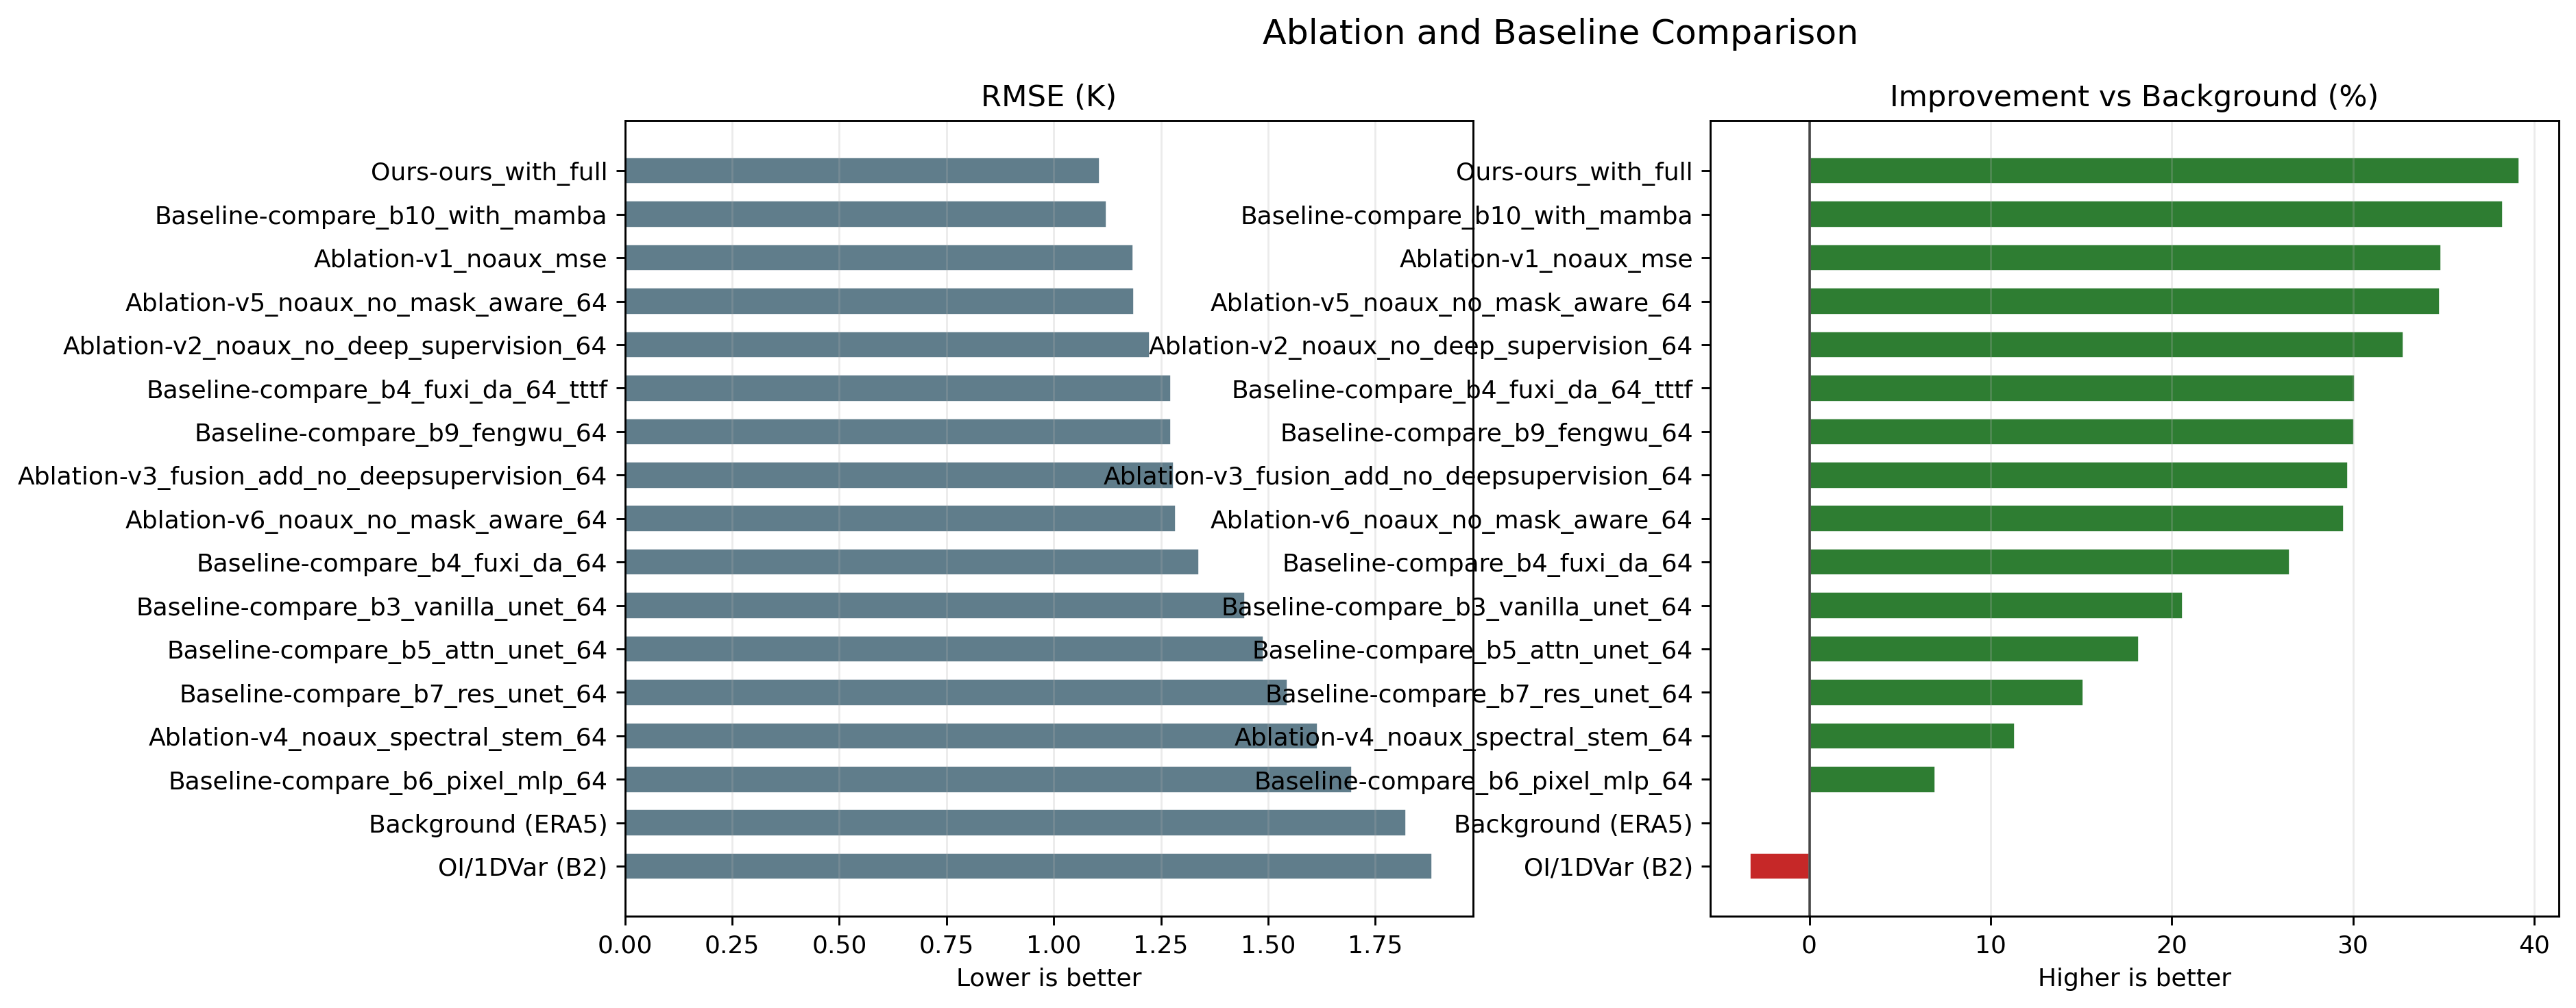
\includegraphics[width=0.9\linewidth]{fig_combined_rmse_improve.png}
\caption{Combined RMSE and improvement comparison.}
\end{figure}

\begin{figure}[htbp]
\centering
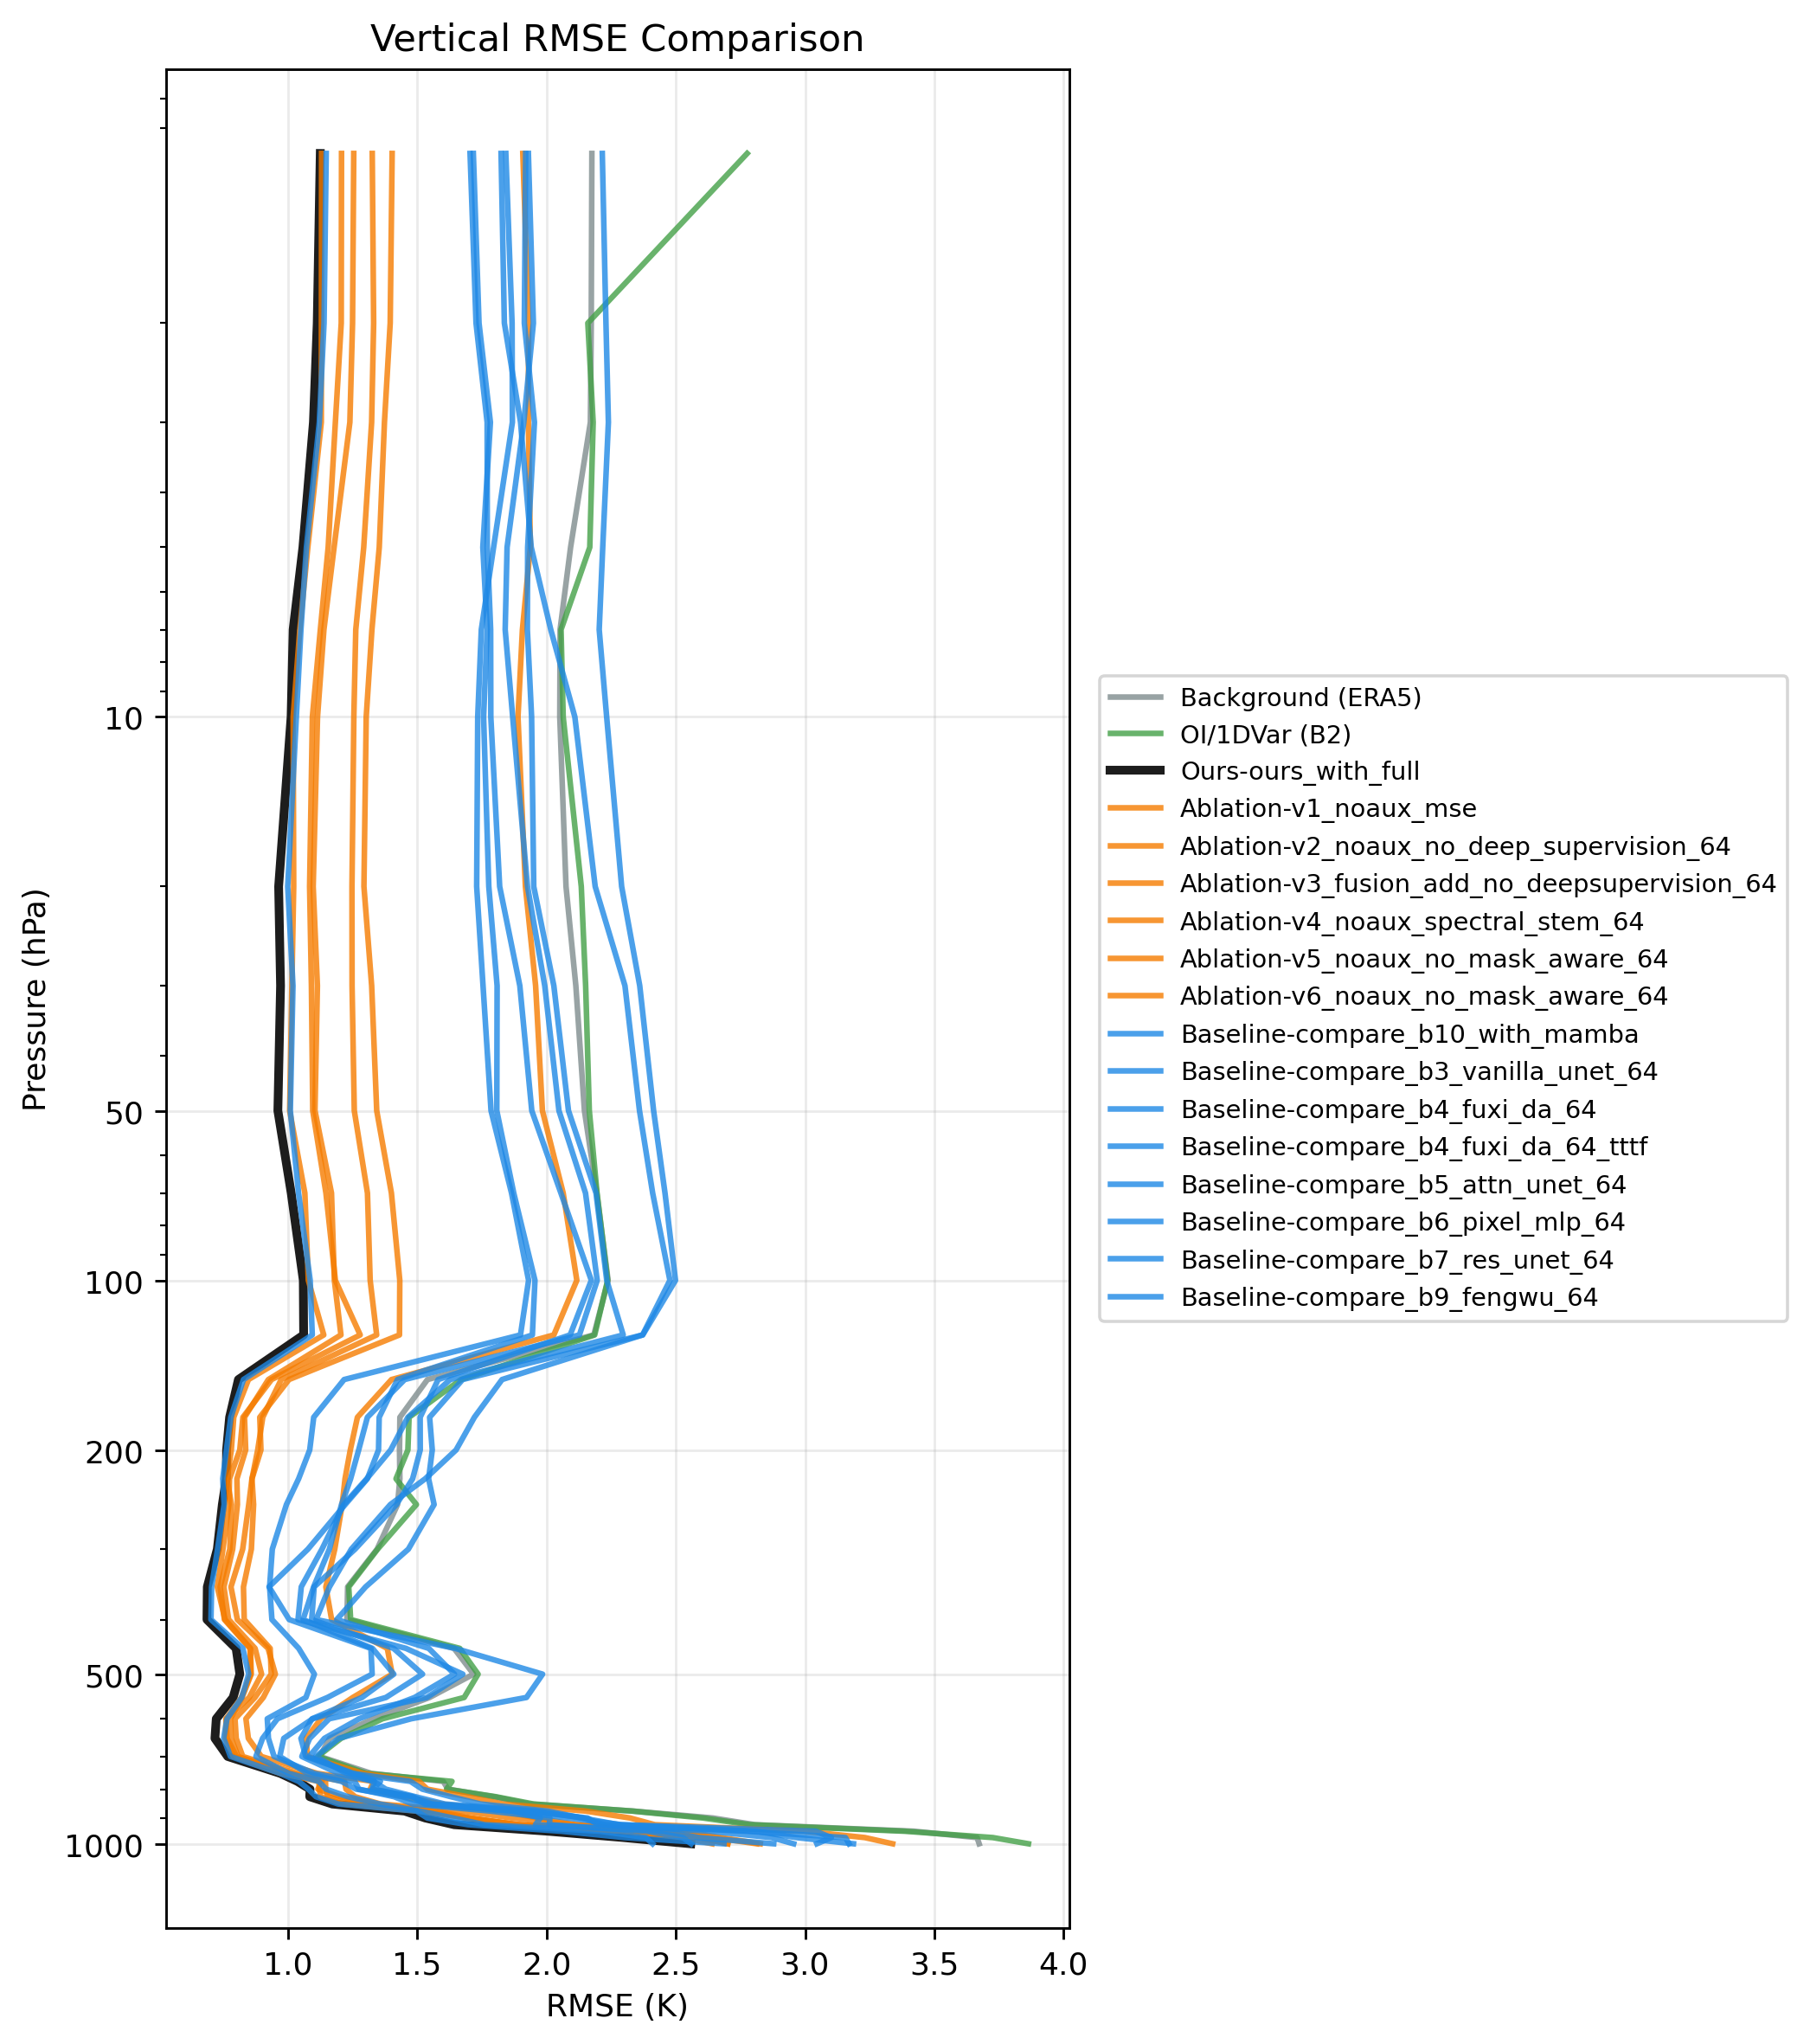
\includegraphics[width=0.9\linewidth]{vertical_rmse_comparison.png}
\caption{Vertical RMSE profiles across pressure levels.}
\end{figure}

\begin{figure}[htbp]
\centering
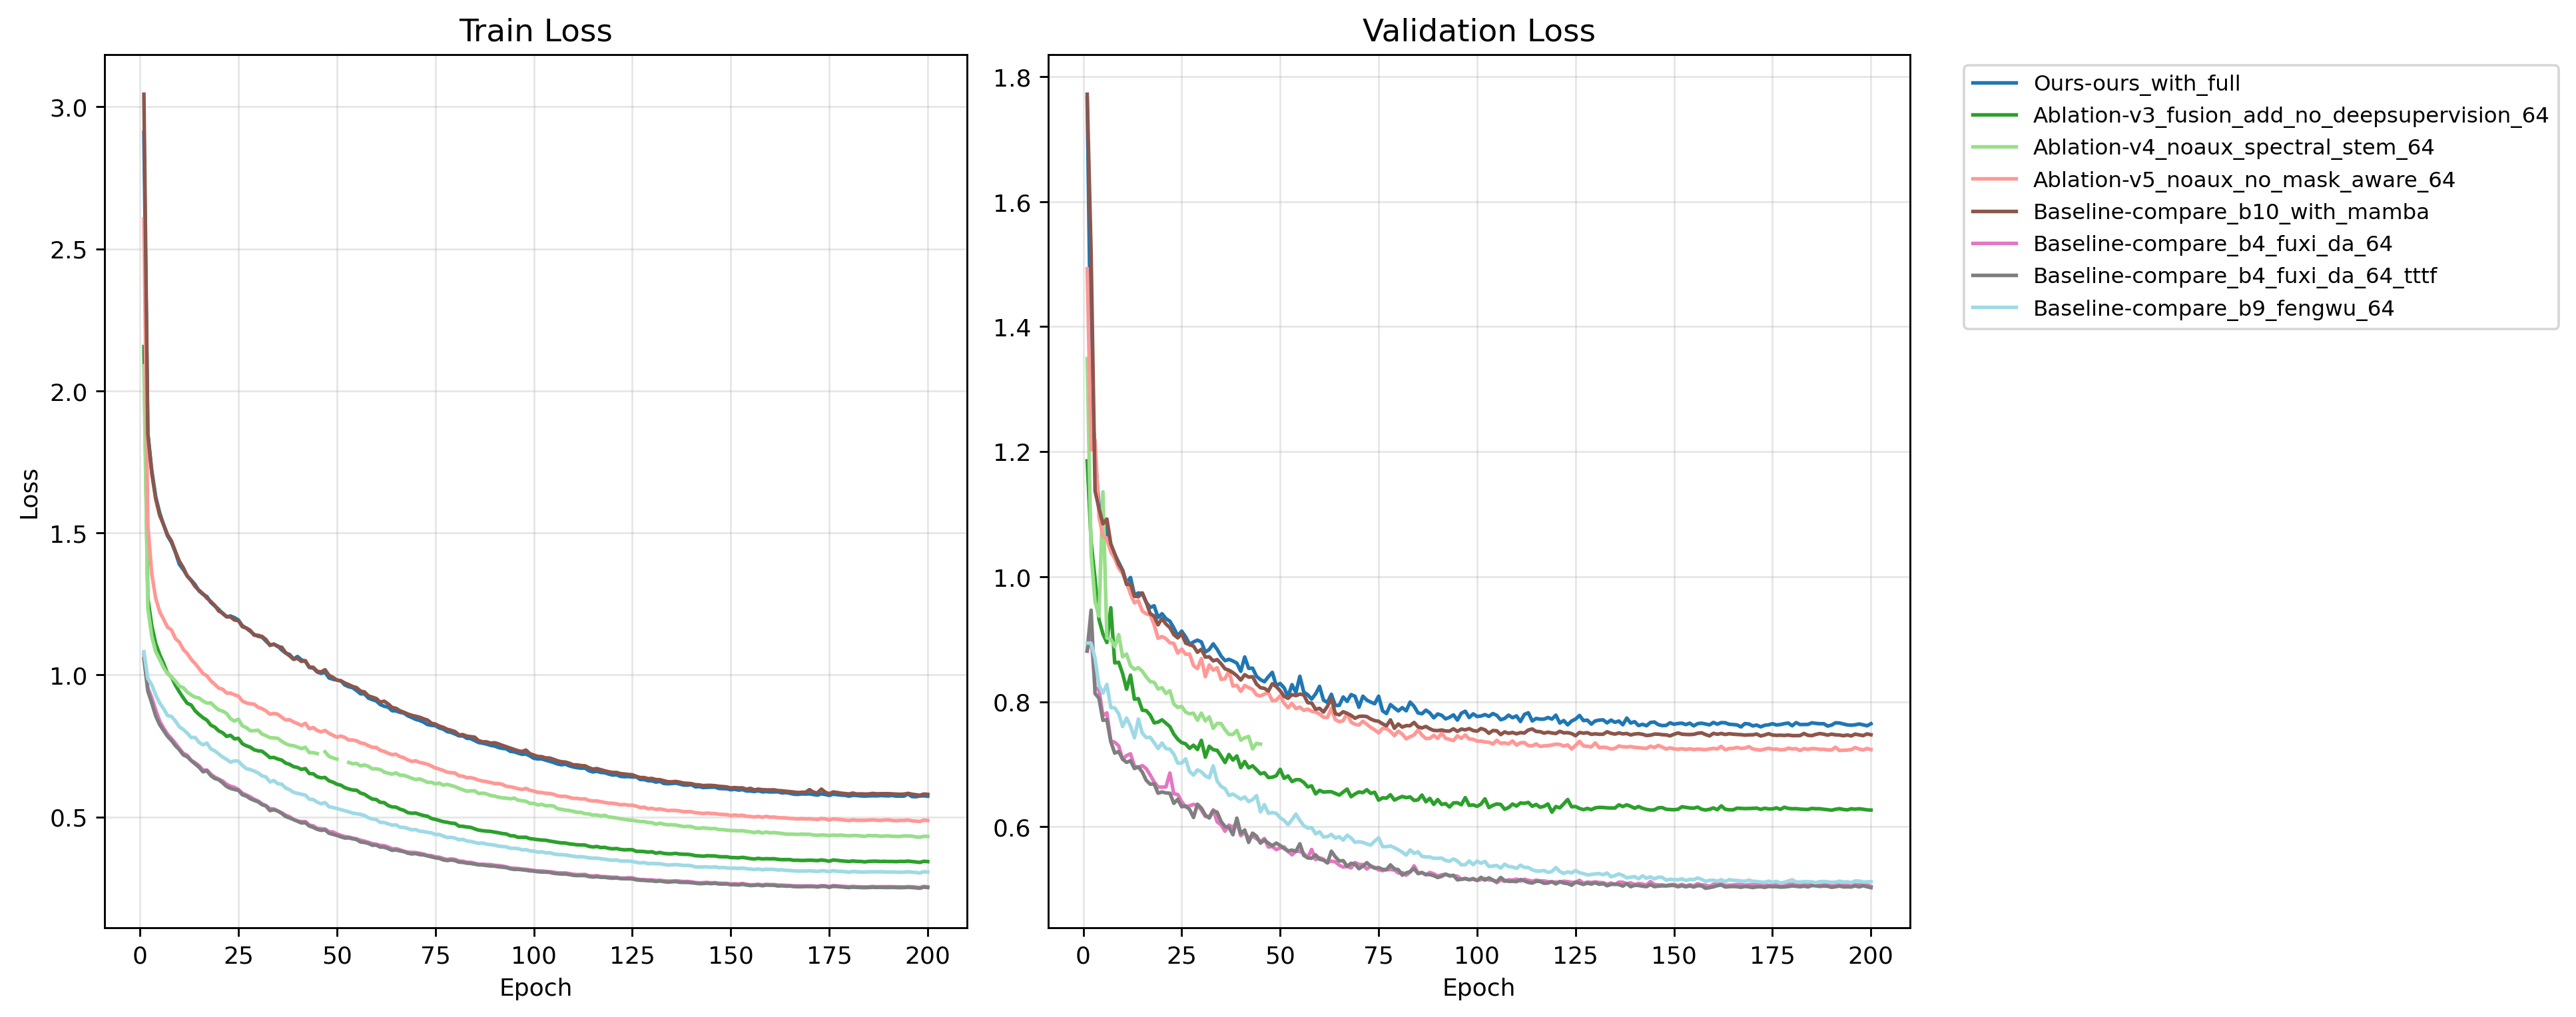
\includegraphics[width=0.9\linewidth]{fig_loss_curves.png}
\caption{Training and validation loss curves.}
\end{figure}

\begin{figure}[htbp]
\centering
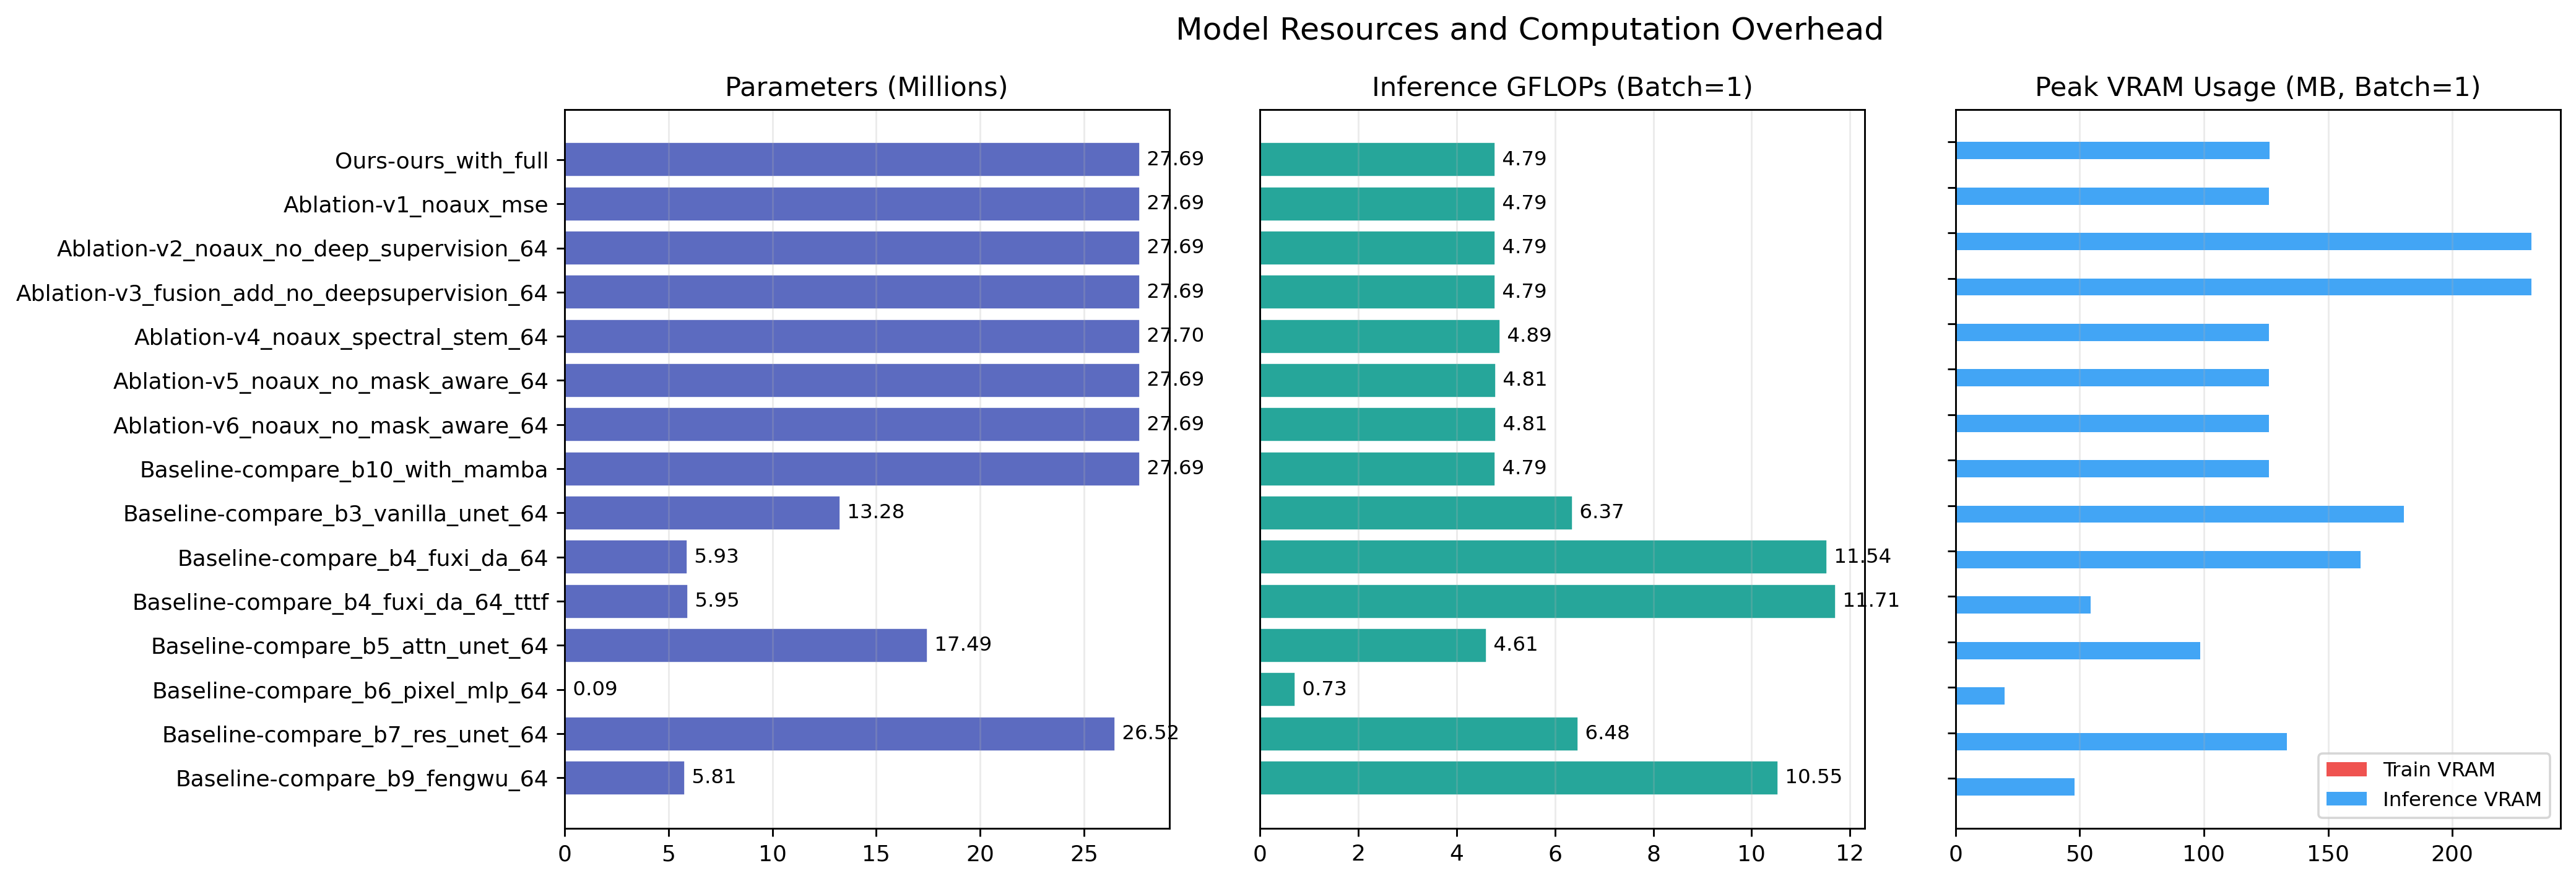
\includegraphics[width=0.9\linewidth]{fig_resources.png}
\caption{Model parameters, GFLOPs, and VRAM usage.}
\end{figure}

\begin{figure}[htbp]
\centering
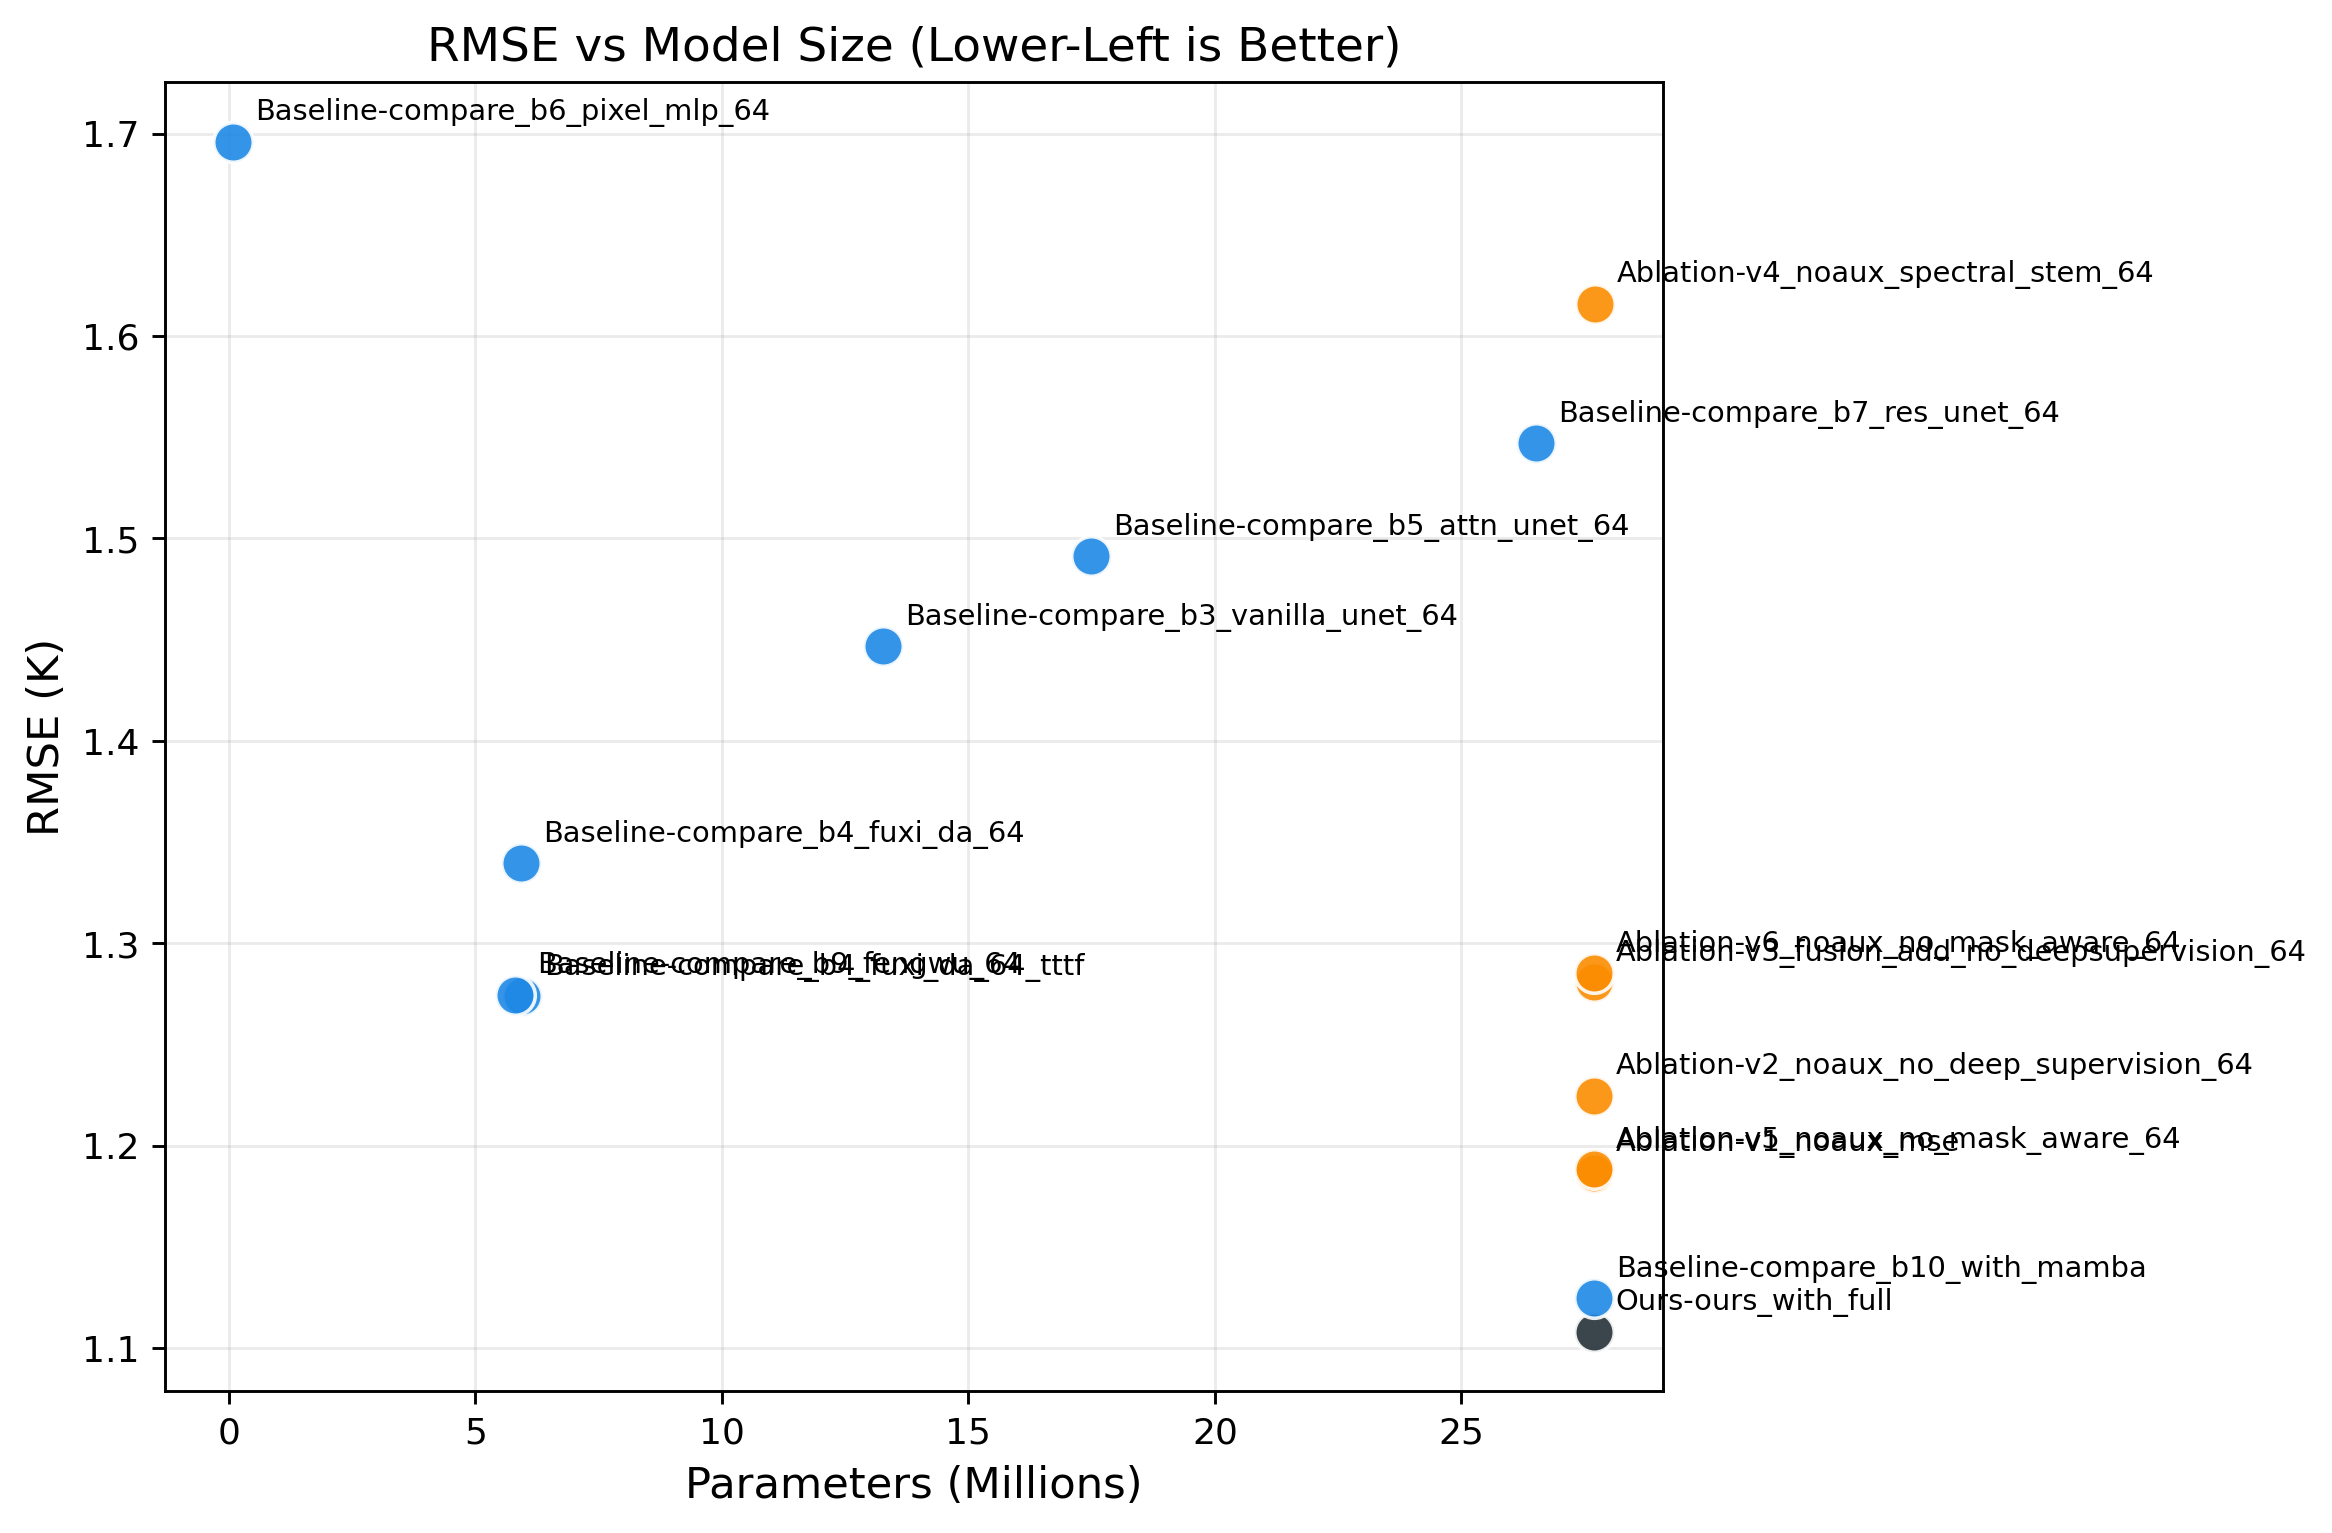
\includegraphics[width=0.9\linewidth]{fig_rmse_vs_params.png}
\caption{RMSE vs model size trade-off.}
\end{figure}

\begin{figure}[htbp]
\centering
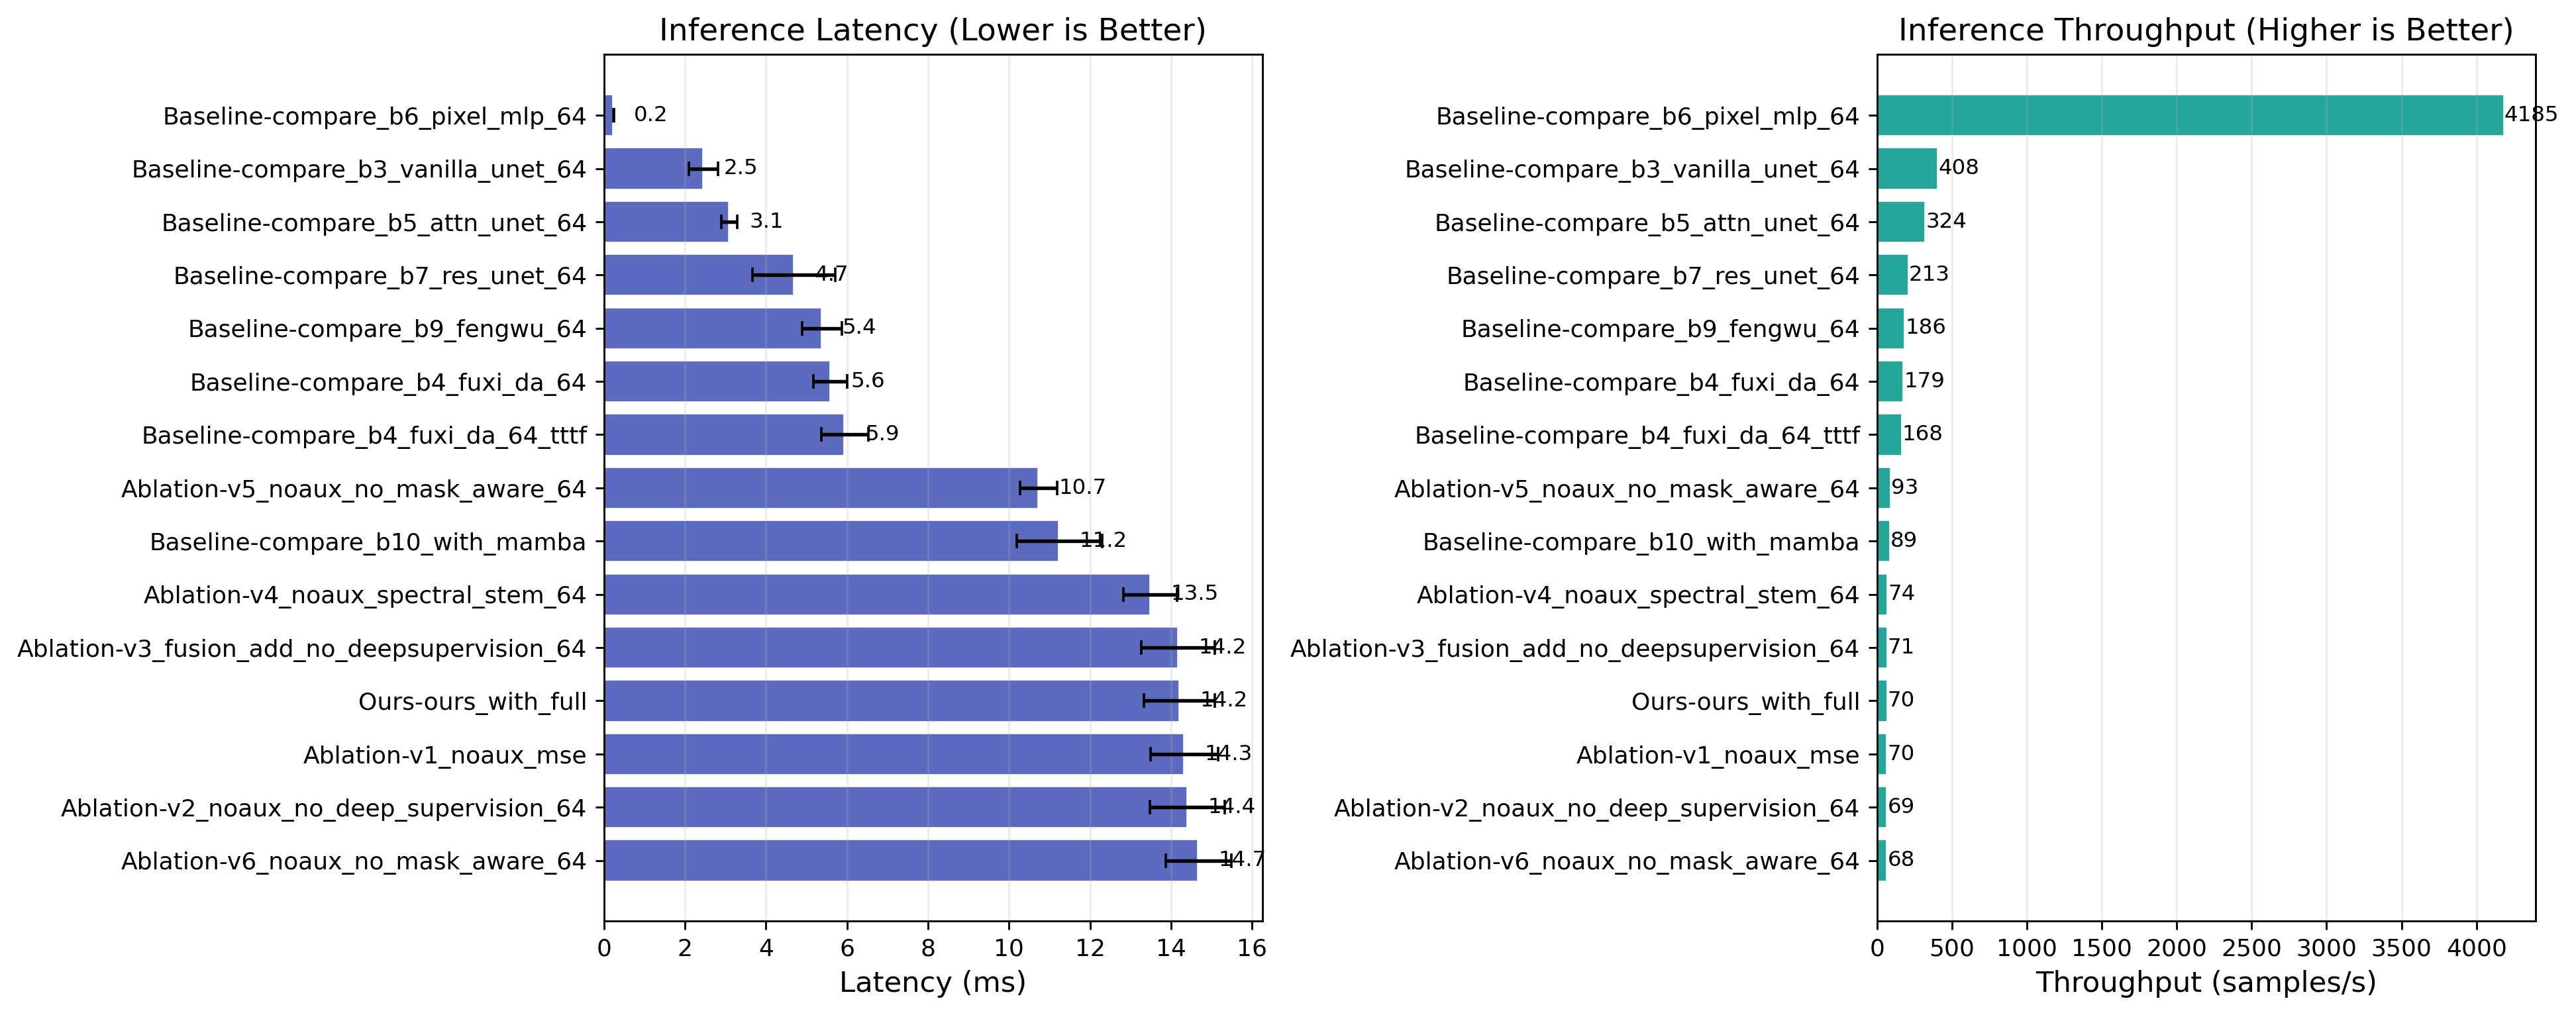
\includegraphics[width=0.9\linewidth]{fig_latency_throughput.png}
\caption{Inference latency and throughput comparison.}
\end{figure}

\begin{figure}[htbp]
\centering
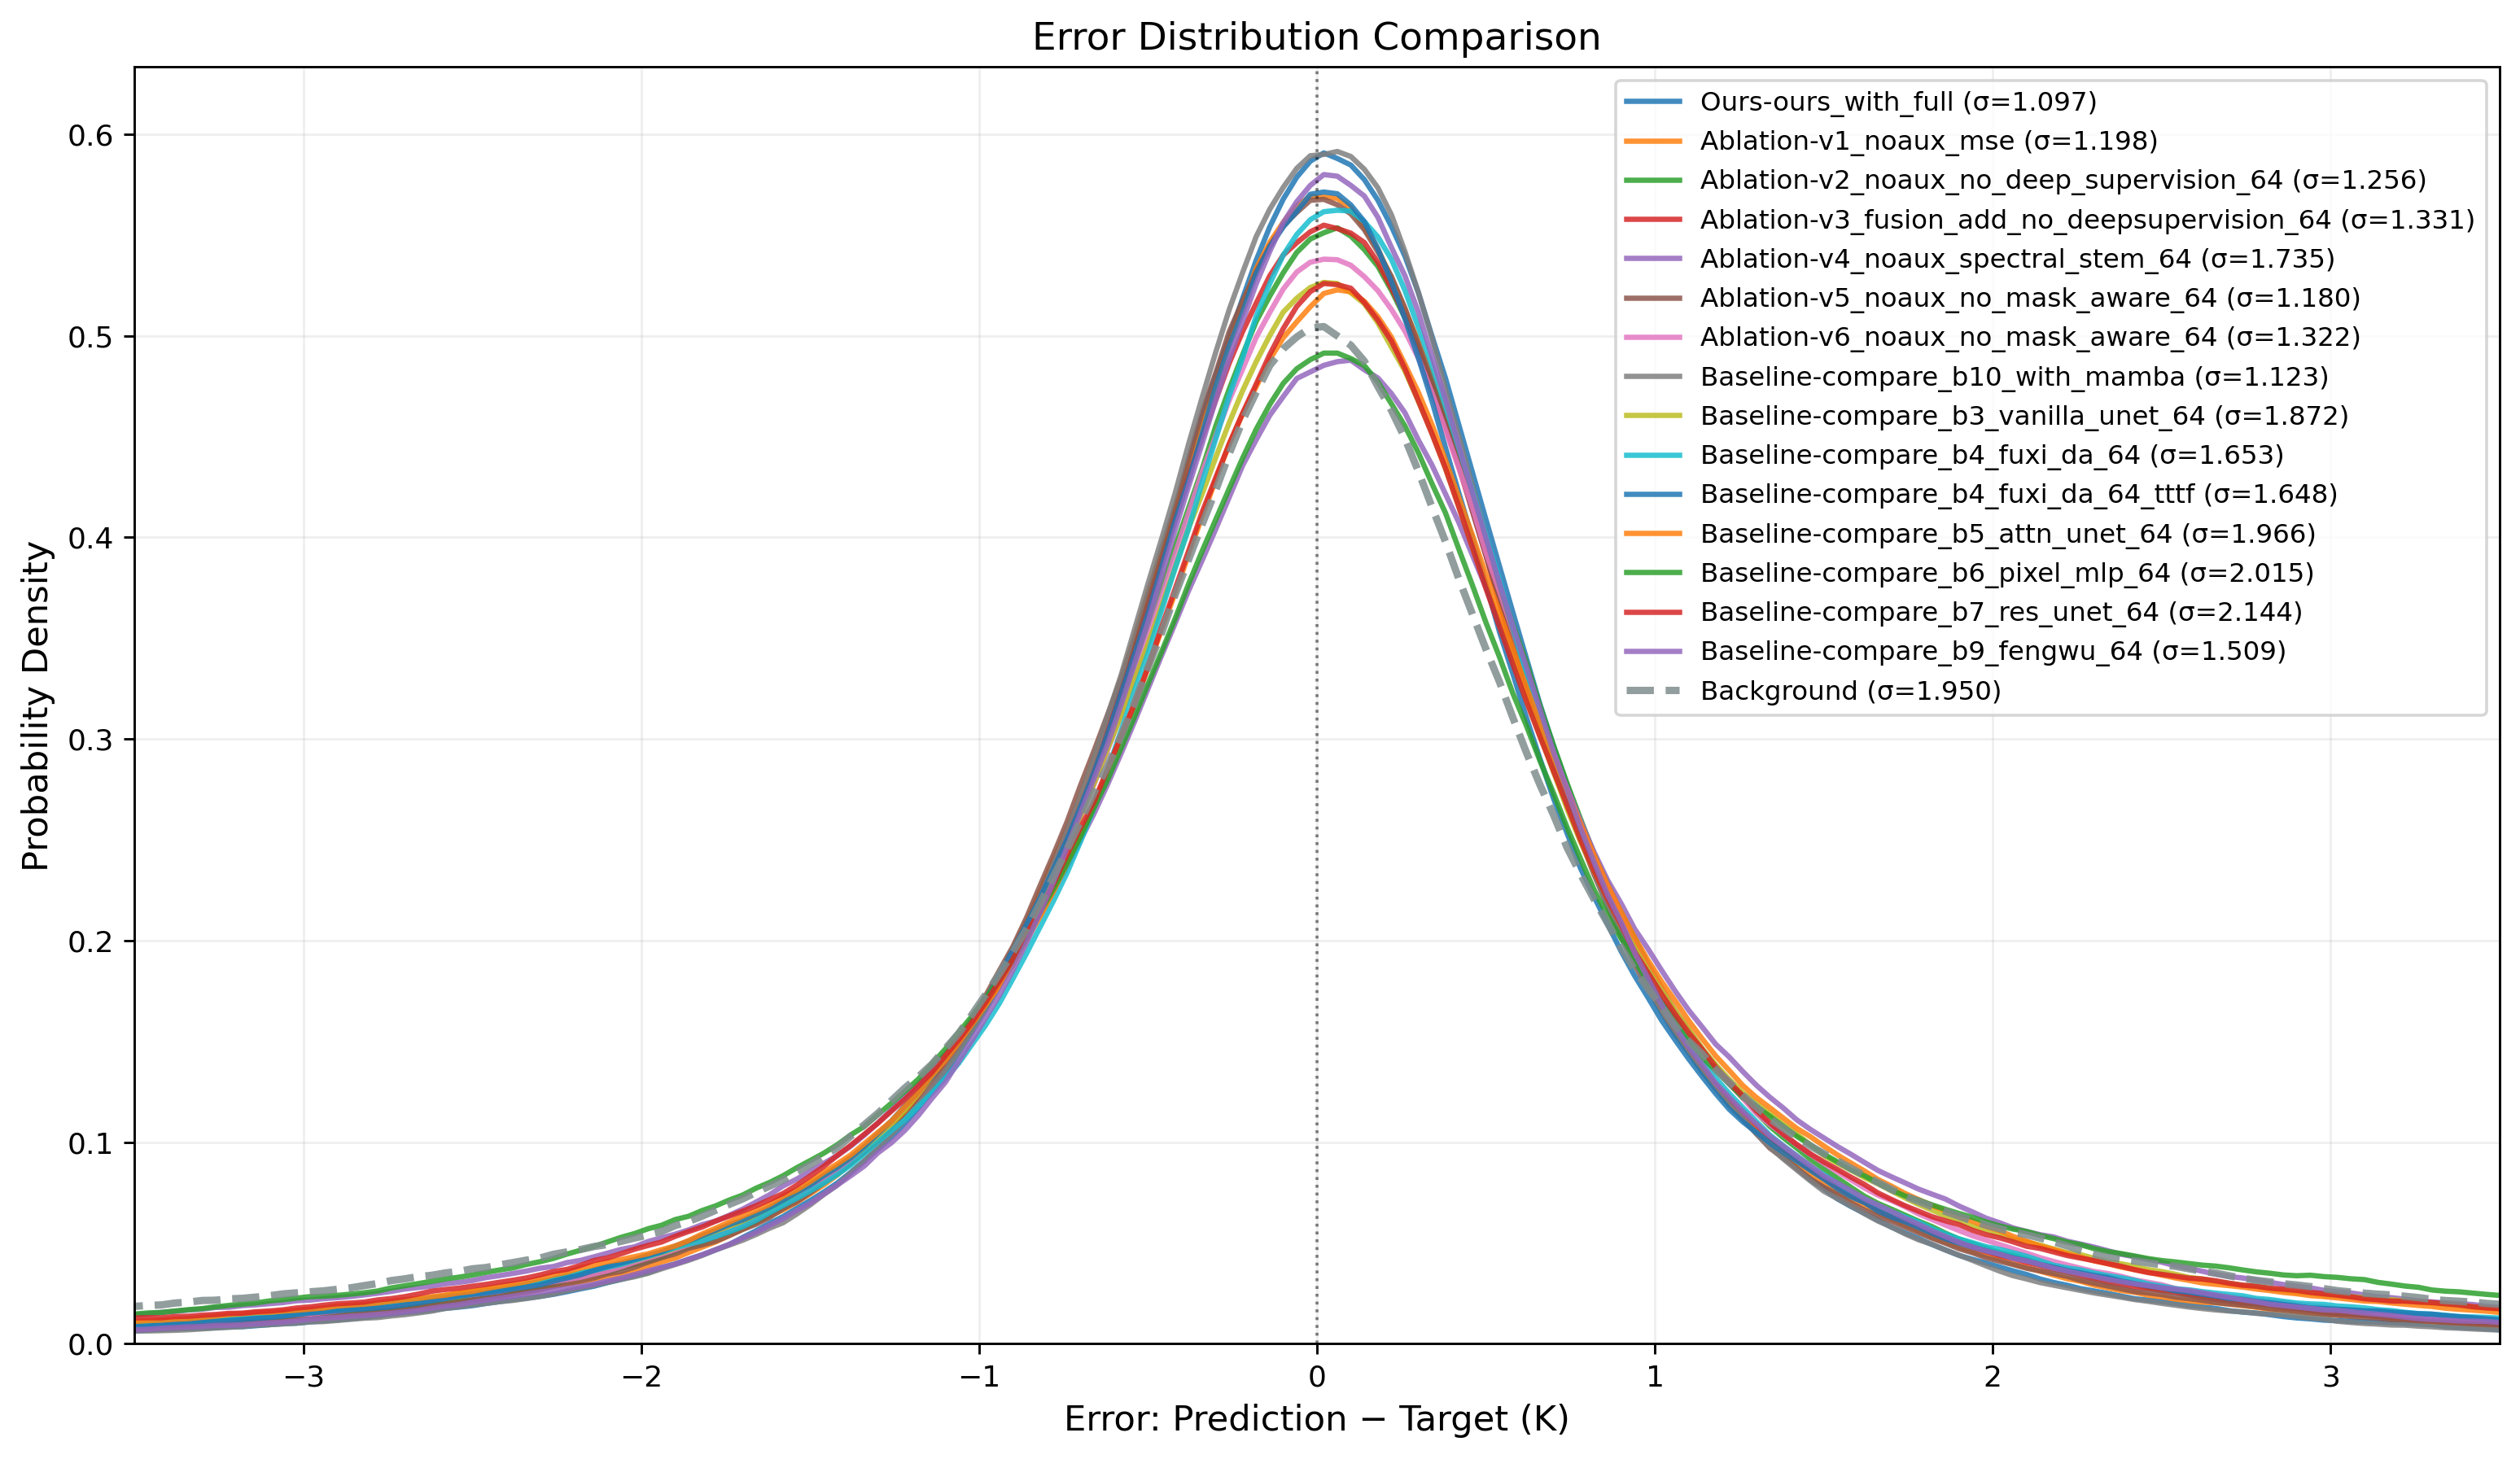
\includegraphics[width=0.9\linewidth]{fig_error_distribution.png}
\caption{Prediction error probability density.}
\end{figure}

\begin{figure}[htbp]
\centering
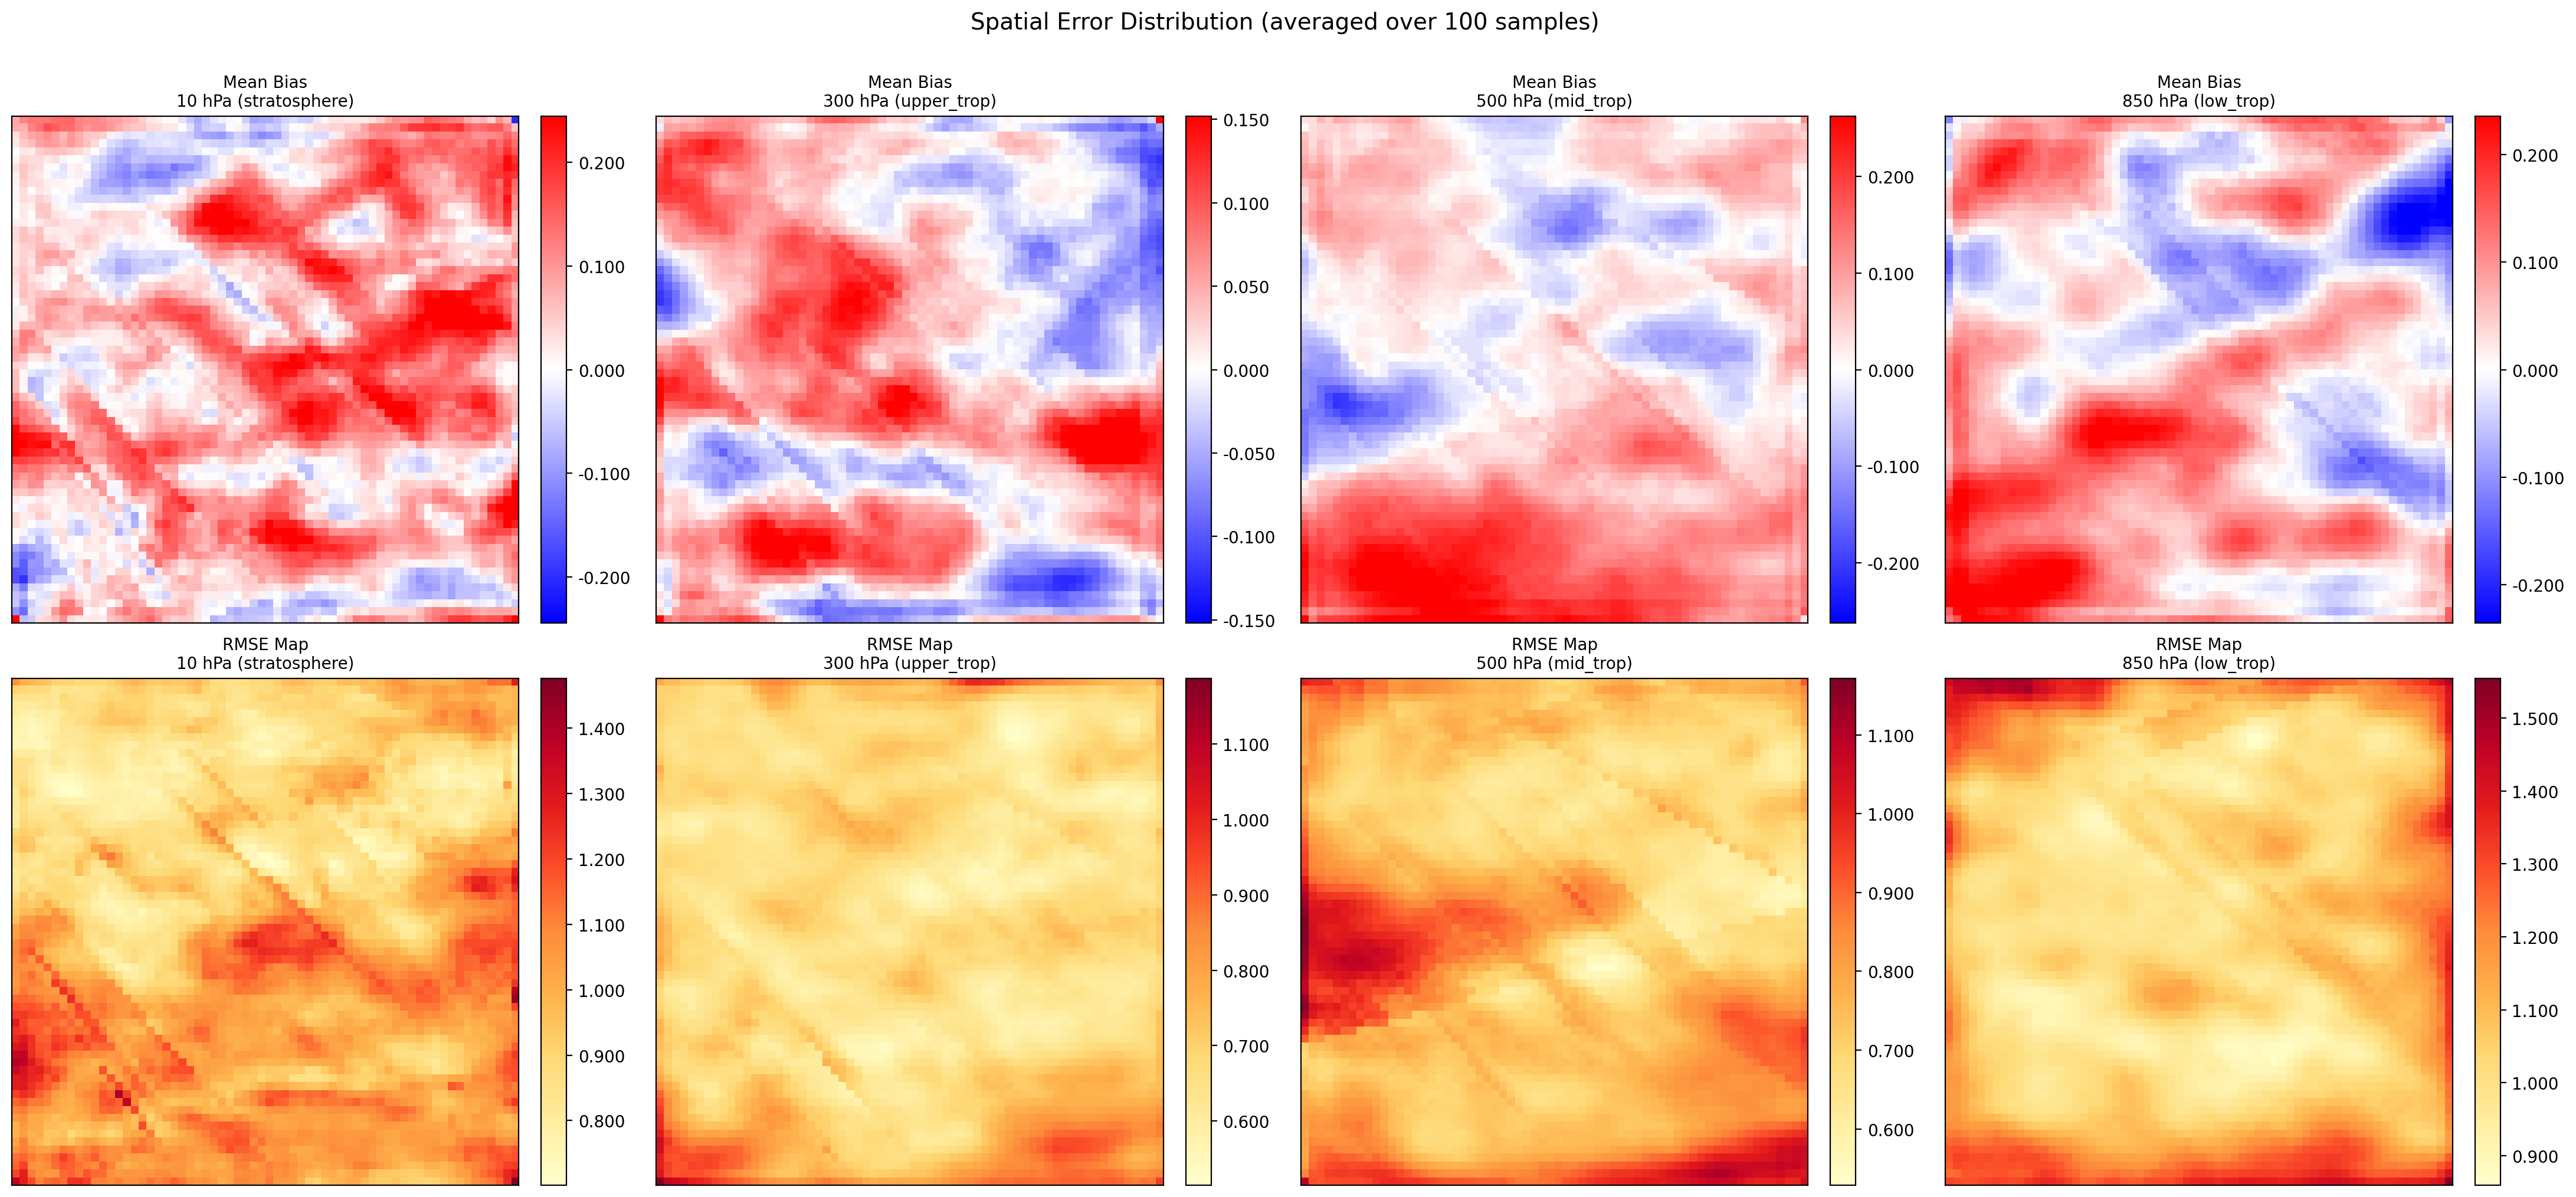
\includegraphics[width=0.9\linewidth]{fig_spatial_error_maps.png}
\caption{Spatial mean bias and RMSE maps at representative levels.}
\end{figure}

\begin{figure}[htbp]
\centering
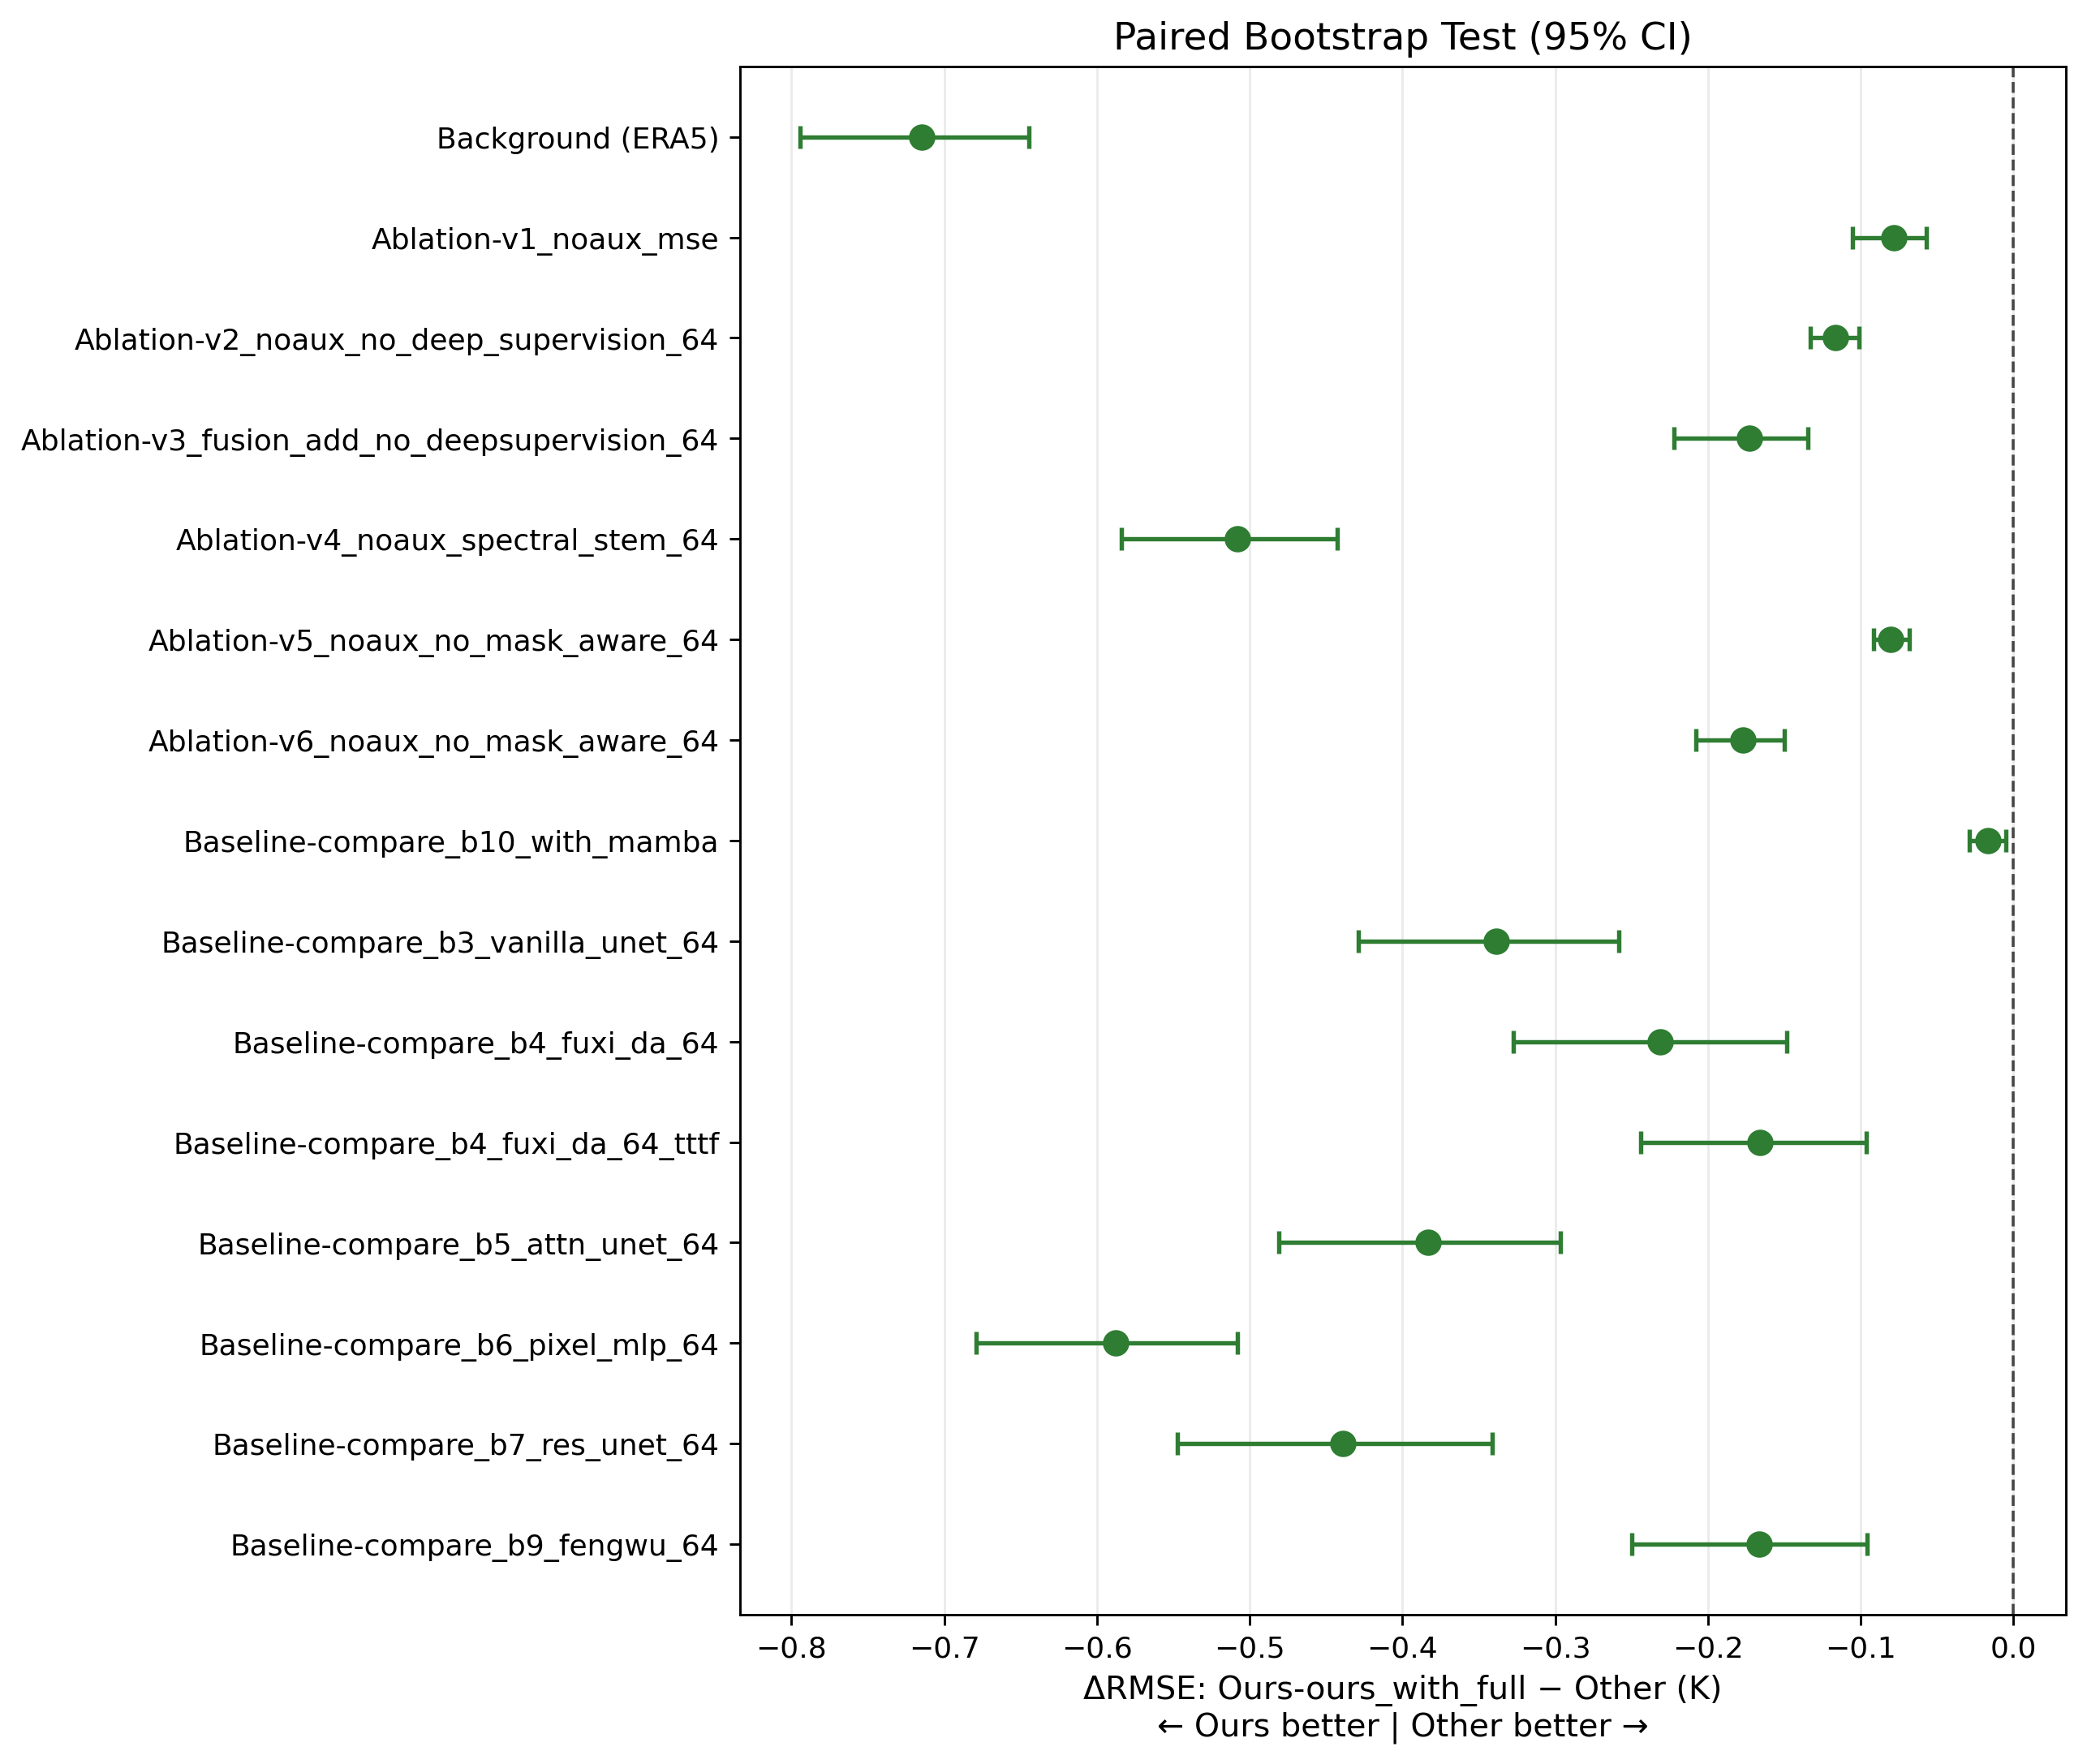
\includegraphics[width=0.9\linewidth]{fig_forest_plot_significance.png}
\caption{Forest plot of paired bootstrap significance tests.}
\end{figure}

\begin{figure}[htbp]
\centering
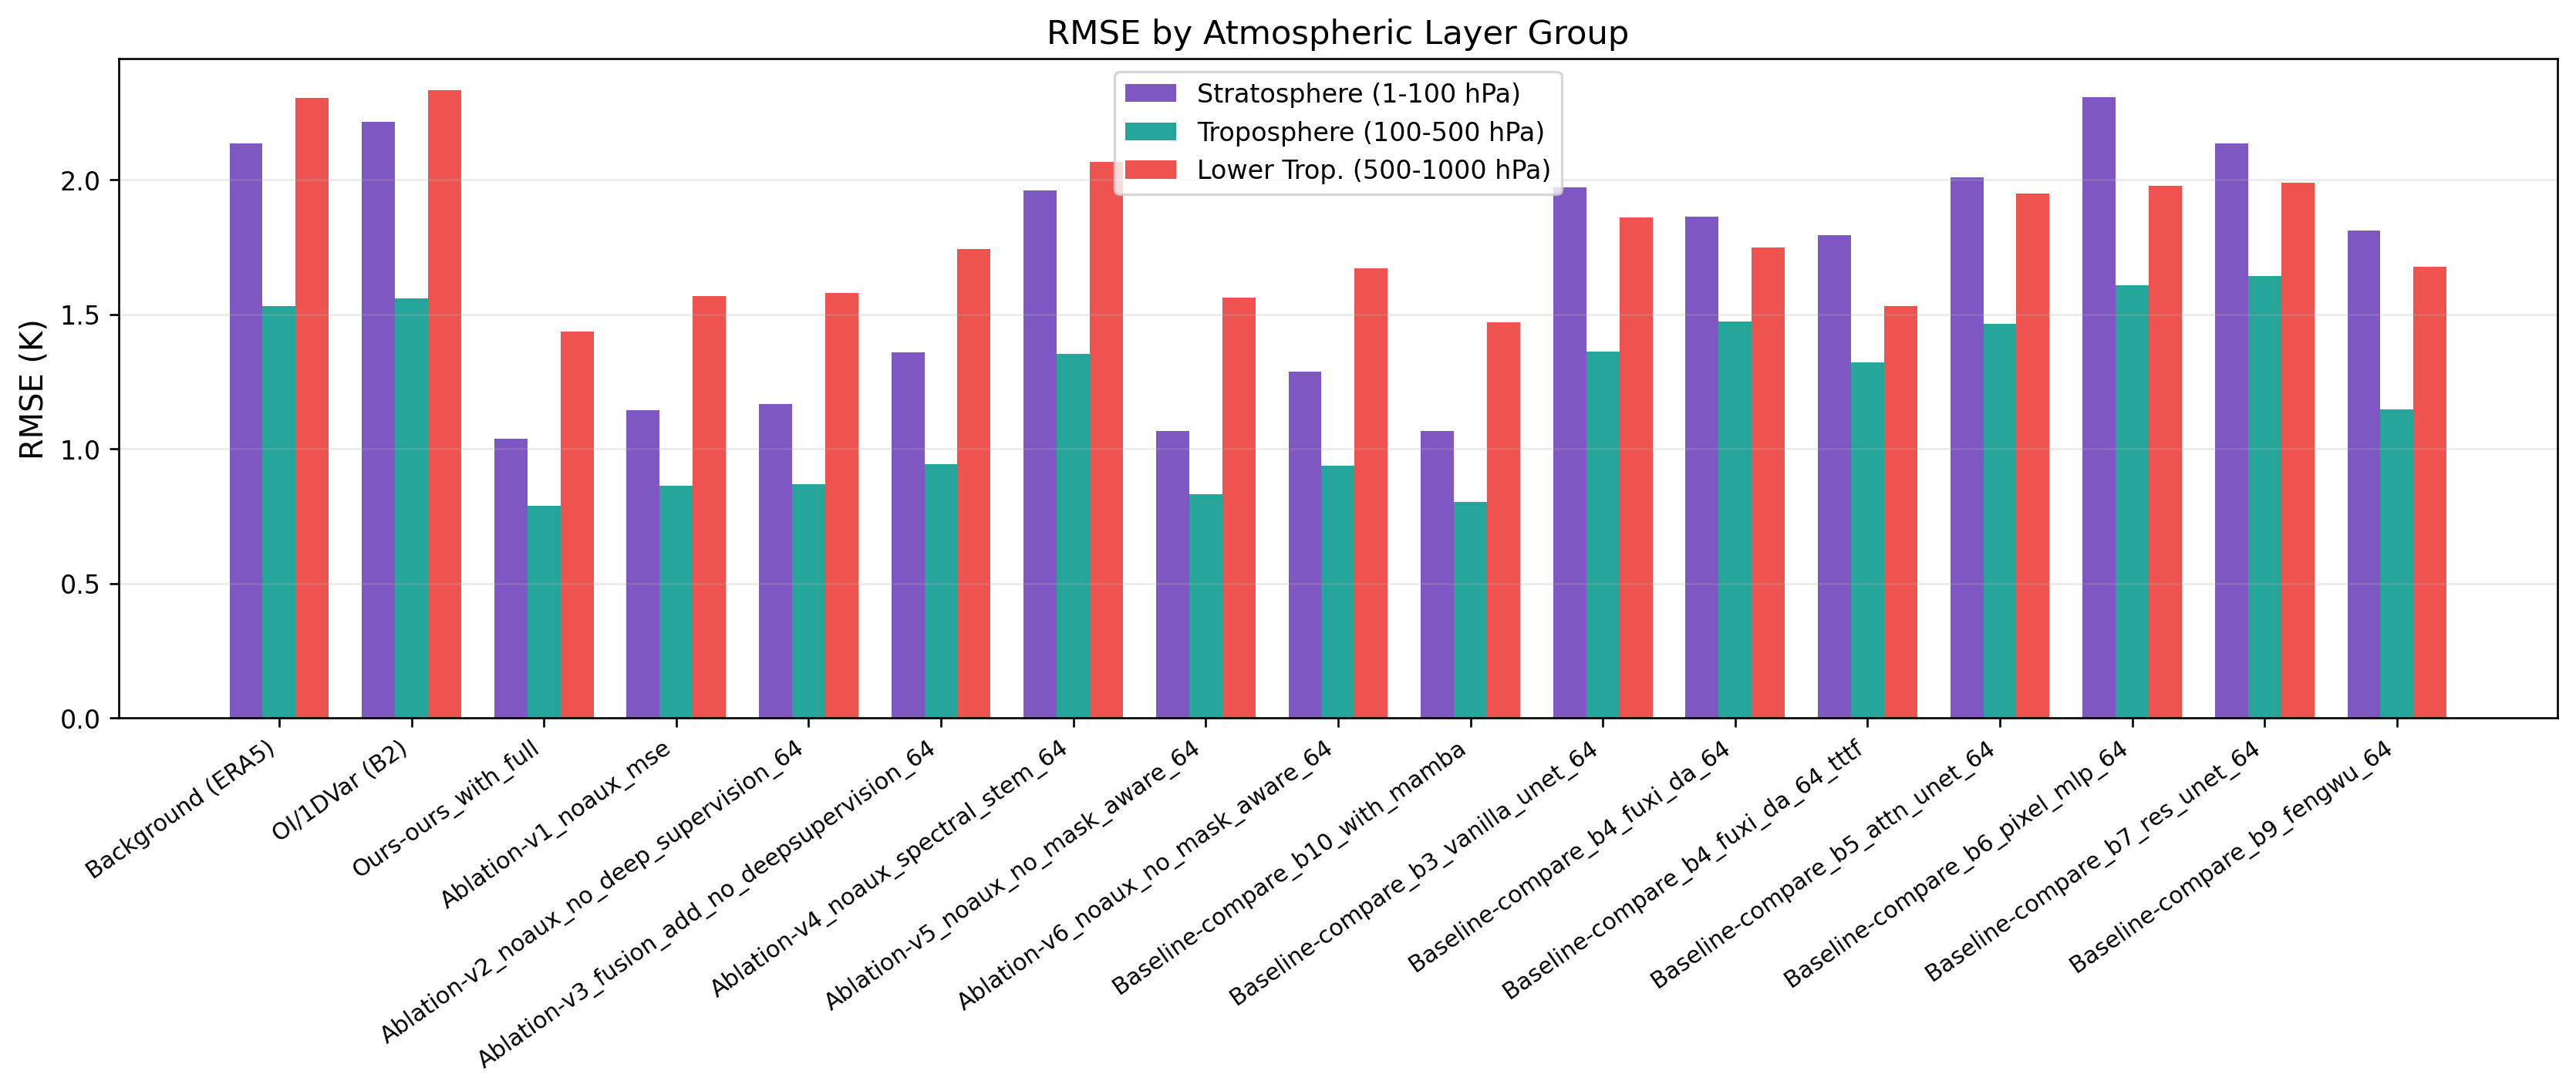
\includegraphics[width=0.9\linewidth]{fig_grouped_rmse_bar.png}
\caption{RMSE breakdown by atmospheric layer group.}
\end{figure}

\section{Conclusion}
See generated figures and tables for detailed analysis.
\end{document}